\documentclass{assignment}

\usepackage{float}
\usepackage{tikz}
\usepackage{adjustbox}
\usepackage{titlesec}
\usepackage{soul}
\usepackage{csvsimple}

\usepackage{bm}
\usepackage{amsmath,amssymb}

\usepackage{pgfplots}
\usepackage{graphics, epsfig}

\usepackage{graphicx}
\usepackage{subcaption}
\usepackage{matlab-prettifier}
\usepackage{multirow}

\usetikzlibrary{decorations.pathmorphing, decorations.markings}
\usetikzlibrary{positioning}

\usetikzlibrary{calc,patterns,angles,quotes}
\setlength{\parindent}{0pt}

\usetikzlibrary{shapes, arrows}
\tikzstyle{startstop} = [rectangle, rounded corners, minimum width=3cm, minimum height=1cm, text centered, draw=black, fill=red!30]
\tikzstyle{io} = [trapezium, trapezium stretches=true, trapezium left angle=70, trapezium right angle=110, minimum width=4cm, minimum height=1cm, text centered, draw=black, fill=blue!30]
\tikzstyle{process} = [rectangle, minimum width=4cm, minimum height=1cm, text centered, text width=4cm, draw=black, fill=orange!30]
\tikzstyle{decision} = [diamond, minimum width=3cm, minimum height=1cm, text centered, draw=black, fill=green!30]
\tikzstyle{arrow} = [thick,->,>=stealth]

\hypersetup{
pdftitle={Autonomous Vehicles},
pdfsubject={Assignment 2},
pdfauthor={Tommaso Bocchietti}
}

\makeglossaries

\begin{document}

\title{Autonomous Vehicles \\ Assignment 2}
\author{Tommaso Bocchietti 10740309}
\date{A.Y. 2024/25}

\maketitle

\begin{figure}[H]
    \centering
    
\includegraphics[width=0.7\textwidth]{./pdf/Polimi_logo_coverpage.pdf}
    \label{fig:Polimi_logo}
\end{figure}

\clearpage
\tableofcontents
\listoffigures
% \listoftables
% \lstlistoflistings
% \printglossary[type=\acronymtype]

\clearpage
\section{Methodology}
\label{sec:methodology}

The aim of this work is to gain insight into the use of \texttt{rosbags} for the analysis of data collected by autonomous vehicles.

The following sections will provide a detailed description of the requests associated with this assignment, the approach taken to fulfill them, and the discussion of the results obtained.

\paragraph{Tools}

As for the tools used, \texttt{ROS1} (Robot Operating System) was employed as the main framework for data collection, while their analysis was performed using \texttt{MATLAB}.
Notice that with the current setup used by the author, \texttt{MATLAB 2024a} was running in Windows 10, while \texttt{ROS1} was running in the \texttt{WSL2} (Windows Subsystem for Linux) environment, specifically in \texttt{Ubuntu 20.04}.

\section{System overview}
\label{sec:system_overview}

In this section, we provide a brief overview of the requests associated with this assignment, along with a description of the approach taken to fulfill them.
In the successive two sections instead, we will provide a detailed description of the control strategies implemented, and the analysis of the results obtained.

\subsection{Request}
\label{subsec:request}

For this assignment, we were asked to implement a feedback control strategy that is able to drive a \texttt{Turtlebot3} robot of the model \texttt{burger} through some predefined waypoints in the environment.

In particular, the waypoints are specified as a list of 3D coordinates in the world frame, where the first two coordinates represent the position of the vehicle in the plane, and the third coordinate represents the orientation of the vehicle in the world frame.
Notice that these data are to be considered as centered in the world frame.

Also, along with this core request, we are asked to implement two control strategy such as:

\begin{itemize}
    \item A simple proportional controller, subjected to a set constraint;
    \item A more advanced controller (no particular constraints on its choice).
\end{itemize}



\subsection{Waypoints}
\label{subsec:waypoints}

Before proceeding with the actual implementation of the control system, we show in Figure \ref{fig:waypoints} the waypoints used for this assignment.
These waypoints were provided along with the text of the assignment.

\begin{figure}[H]
    \centering
    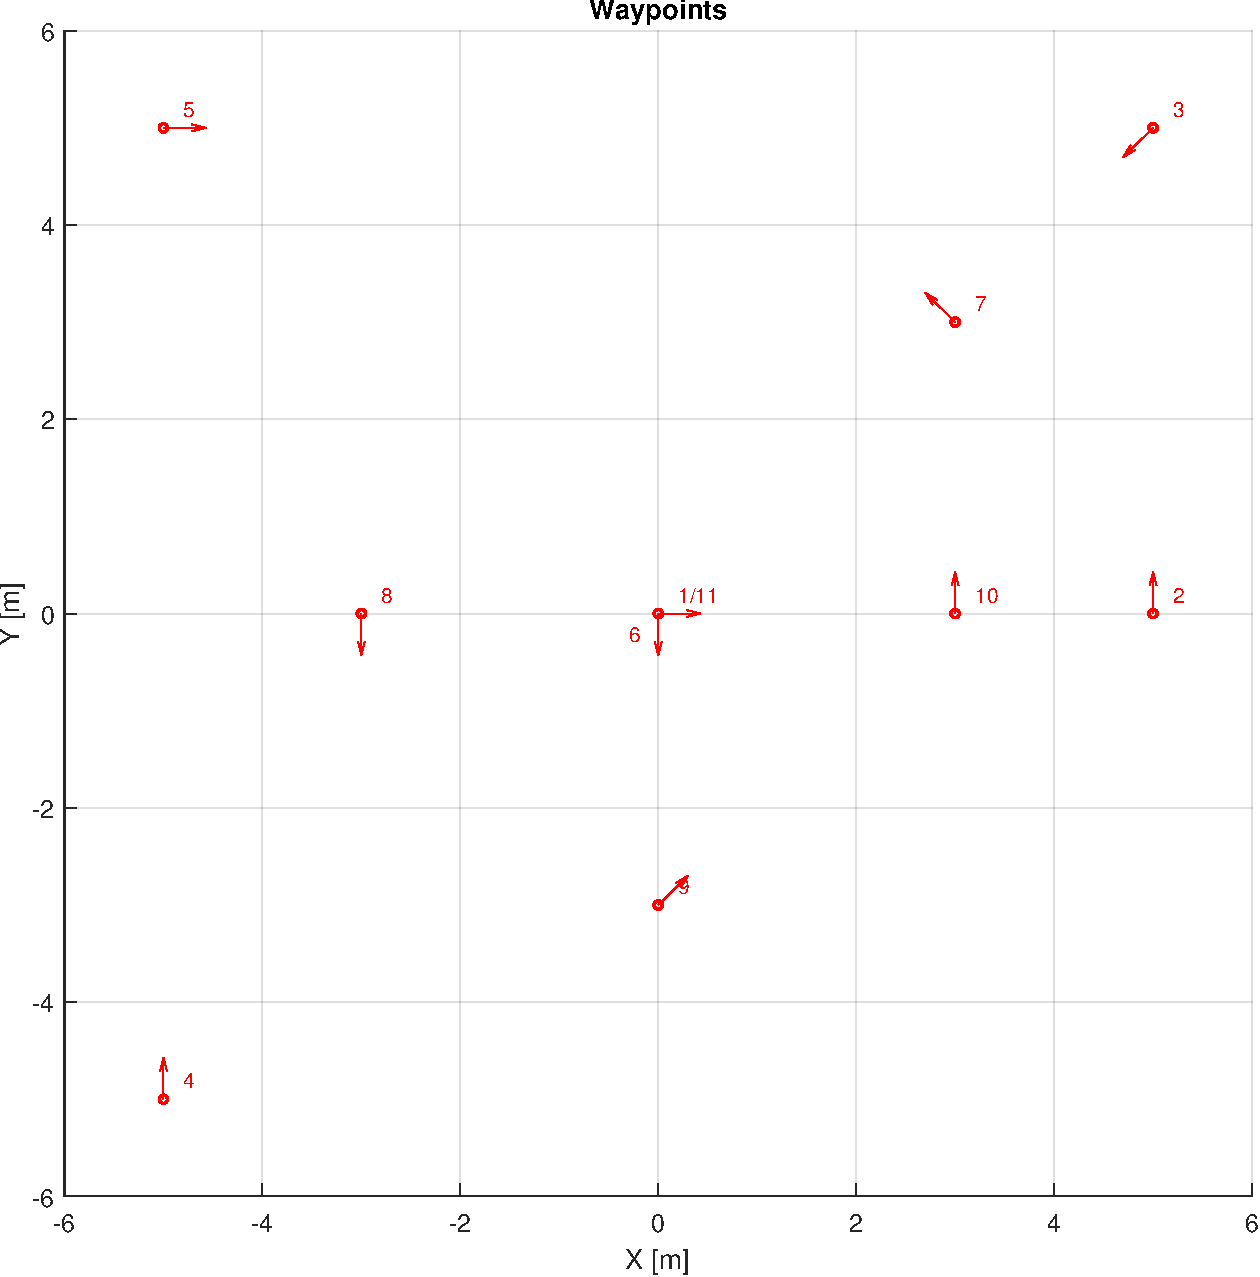
\includegraphics[width=0.6\textwidth]{./img/MATLAB/waypoints.pdf}
    \caption{Waypoints used for the simulation.}
    \label{fig:waypoints}
\end{figure}

In Figure \ref{fig:waypoints}, we can see the waypoints used for the simulation, which are represented as red dots in the world frame.
The arrow associated to each waypoint represents the orientation of the vehicle at that waypoint, which is given by the third coordinate of the waypoint list.



\subsection{Simulink model}
\label{subsec:simulink_model}

As already mentioned in the previous section, the logic of the feedback control system was implemented in \texttt{Simulink}, which is a graphical programming environment for modeling, simulating and analyzing dynamic systems.
In Figure \ref{fig:simulink_model} we can see the Simulink model used for this assignment.

\begin{figure}[H]
    \centering
    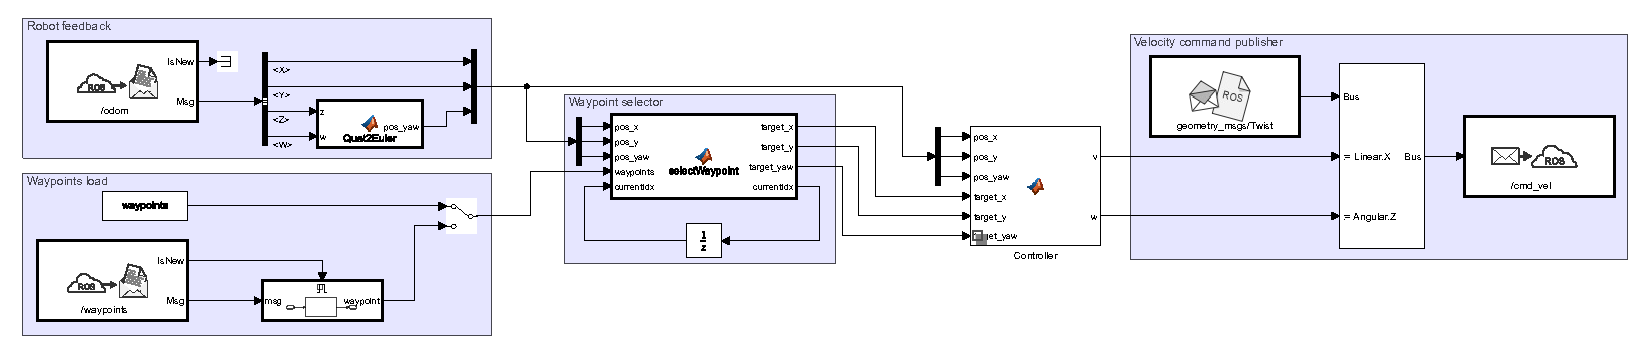
\includegraphics[width=1.0\textwidth]{./img/MATLAB/overview.pdf}
    \caption{Simulink model used for the implementation of the feedback control system.}
    \label{fig:simulink_model}
\end{figure}

One can easily recognize the different components of the system thanks to the colored areas used to group the different blocks.
The main components of the system are:

\begin{itemize}
    \item Sensors readings: these blocks are used to subscribe to the \texttt{/odom} topic and to extract the data needed for the control system;
    \item Waypoint loader: this block is used to load the waypoints from either a workspace variable or a custom topic \texttt{/waypoints} on which the list of waypoints is published;
    \item Waypoint selector: this block is used to select the current waypoint from the list of waypoints, based on the current position of the vehicle and its history;
    \item Controller: this block is used to implement the feedback control system, which is responsible for computing the control commands to be sent to the vehicle based on the current position and orientation of the vehicle, and the current waypoint to be reached. More details on the implementation of the controller will be provided in the next sections;
    \item Command publisher: this block is used to publish the control commands to the \texttt{/cmd\_vel} topic, which is used by the vehicle to receive the control commands.
\end{itemize}

Notice that the commands sent to the vehicle are comprehensive of both linear and angular velocities, given that the \texttt{burger} model is a differential drive robot.

Inside the controller block, we can find the two different control strategies implemented for this assignment, namely a simple proportional controller and a more advanced controller based on Lyapunov stability theory.
See Figure \ref{fig:controller_block} for an inside view of the controller block.

\begin{figure}[H]
    \centering
    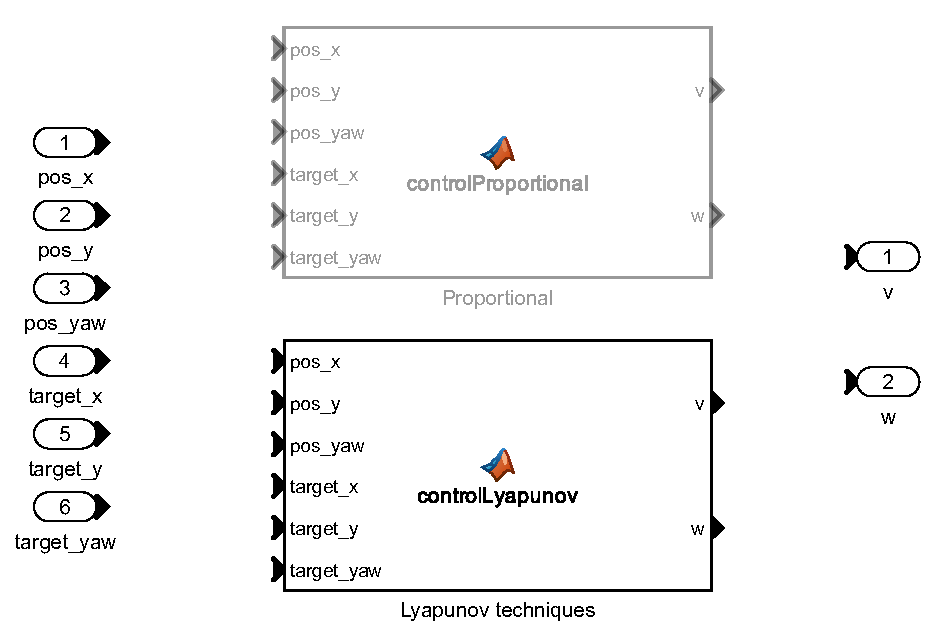
\includegraphics[width=0.9\textwidth]{./img/MATLAB/controller.pdf}
    \caption{Inside view of the controller block.}
    \label{fig:controller_block}
\end{figure}

\section{Proportional controller}
\label{sec:proportional_controller}

As explained in the previous section, one of the requests associated with this assignment is to implement a simple proportional controller for the \texttt{Turtlebot3} robot.

For this task, we have opted for a simple two-stage proportional controller.
In particular, based on the distance of the robot from the current target waypoint, we apply a control input so that:

\begin{itemize}
    \item If the robot is far from the target waypoint, we force its direction to be aligned with the target position, and we apply a linear velocity proportional to the distance from the target;
    \item Instead, when the robot is close to the target waypoint, we apply a control input that forces the robot to rotate in place, so that it can align its direction with the direction required by the target waypoint.
\end{itemize}

Some control constraints are also applied.
In particular, we limit the maximum linear velocity to $0.2 \text{ [m/s]}$ and the maximum angular velocity to $0.4 \text{ [rad/s]}$.
Moreover, we consider the robot to be close to the target waypoint when the Euclidean distance from the target waypoint is less than $0.05 \text{ [m]}$.



\subsection{Implementation}
\label{subsec:implementation_proportional_controller}

The code for the implementation of the controller is provided in the Listing \ref{lst:proportional_controller_code}.

\begin{lstlisting}[
    style=Matlab-editor,
    caption={Code for the implementation of the proportional controller.},
    label={lst:proportional_controller_code}
]
function [v, w] = controlProportional(pos_x, pos_y, pos_yaw, target_x, target_y, target_yaw)
% This controller align the robot with the target waypoint and guide it to
% reach it. Once within the threshold zone, correct the yaw of the robot.
% It uses simple Proportional controller for both actions.

bound = @(value, limit) max(min(value, limit), -limit);

% Gains
K_v = 1.2;
K_w = 1.5;
max_linear_speed = 0.2;
max_angular_speed = 0.4;

dx = target_x - pos_x;
dy = target_y - pos_y;
dist_to_target = hypot(dx, dy);
angle_to_target = atan2(dy, dx);

% Control logic
if dist_to_target > 0.05
    v = K_v * dist_to_target;
    w = K_w * wrapToPi(angle_to_target - pos_yaw);
else
    v = 0;
    w = K_w * wrapToPi(target_yaw - pos_yaw);
end

v = bound(v, max_linear_speed);
w = bound(w, max_angular_speed);

end
\end{lstlisting}



\subsection{Results}
\label{subsec:results_proportional_controller}

Given the above implementation of the proportional controller, we can now analyze the results obtained during the simulation.

The results of the obtained trajectory are shown in Figure \ref{fig:proportional_controller_trajectory}, where we report the waypoints highlighted in red and the trajectory of the robot drawn in black.

\begin{figure}[H]
    \centering
    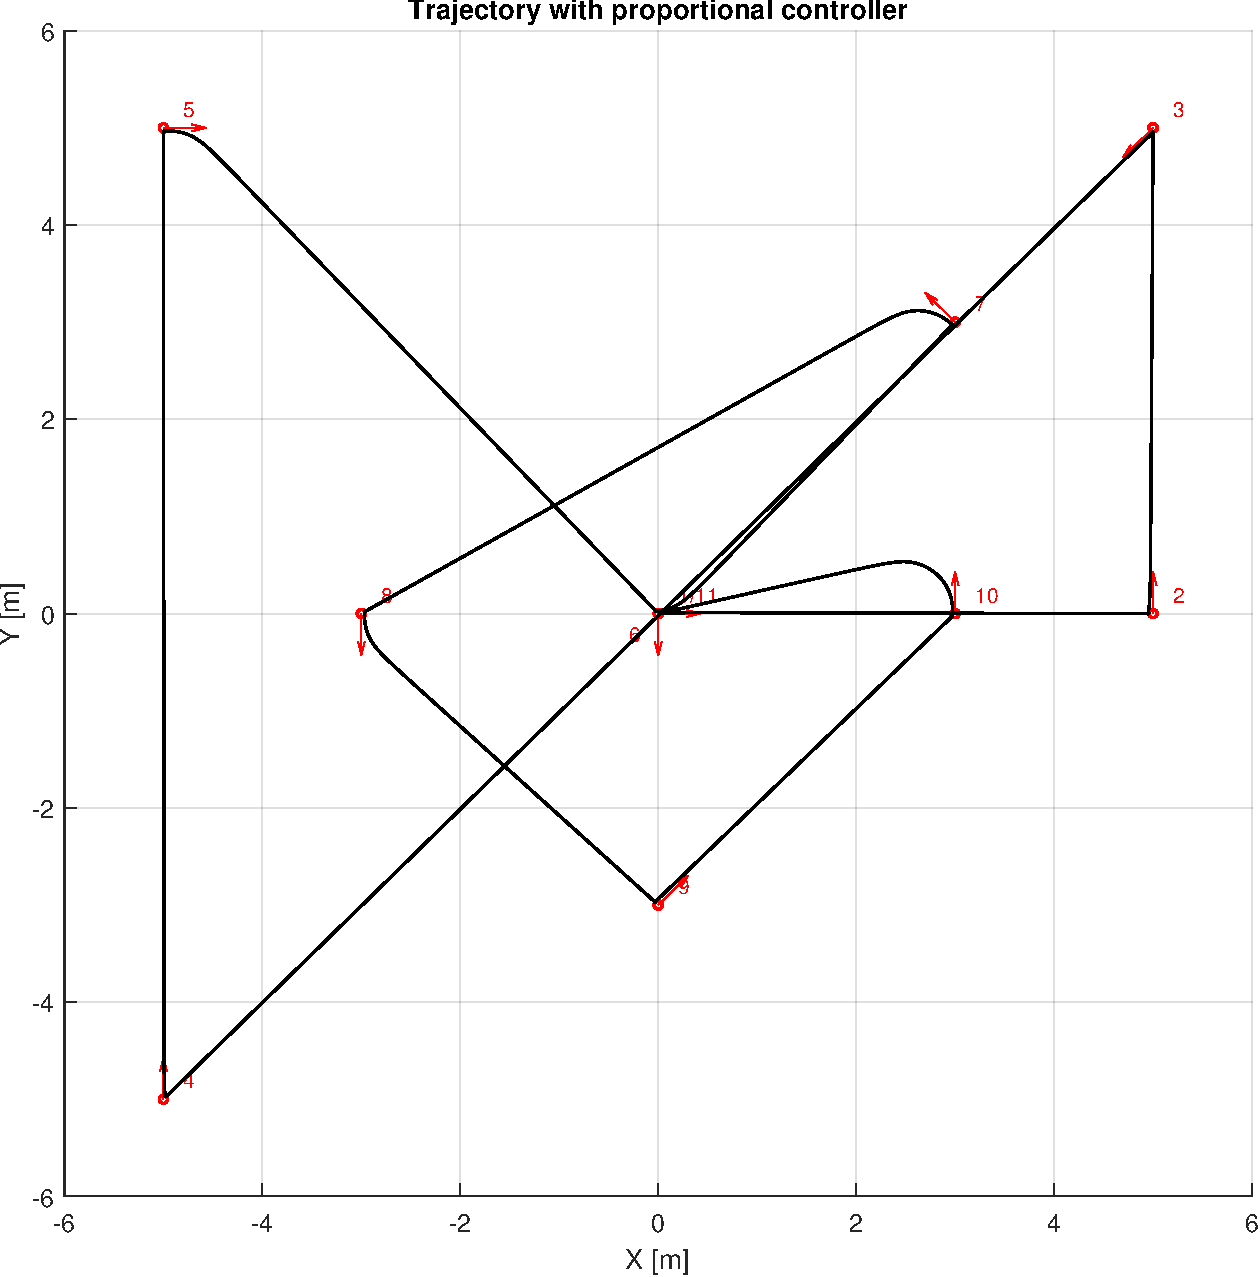
\includegraphics[width=0.6\textwidth]{./img/MATLAB/trajectory_proportional.pdf}
    \caption{Trajectory of the robot during the simulation with the proportional controller.}
    \label{fig:proportional_controller_trajectory}
\end{figure}

One can easily observe that all the waypoints have been reached successfully.

When it comes to the velocity profiles, both in linear and angular dimension, it's easy to visualize the constraints applied to the controller.
The linear velocity is limited to $0.2 \text{ [m/s]}$, while the angular velocity is limited to $0.4 \text{ [rad/s]}$.
This results in a trapezoidal profile for the velocities, as shown in Figure \ref{fig:proportional_controller_velocity_profiles}.

\begin{figure}[H]
    \centering
    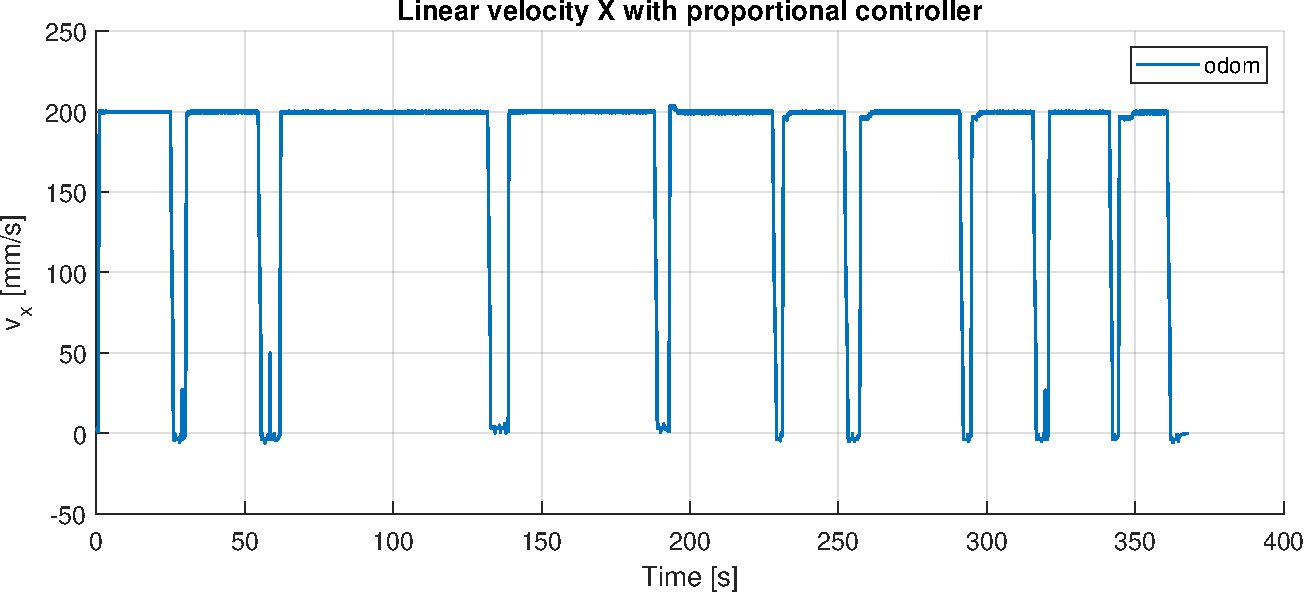
\includegraphics[width=0.7\textwidth]{./img/MATLAB/linear_velocity_proportional.pdf}
    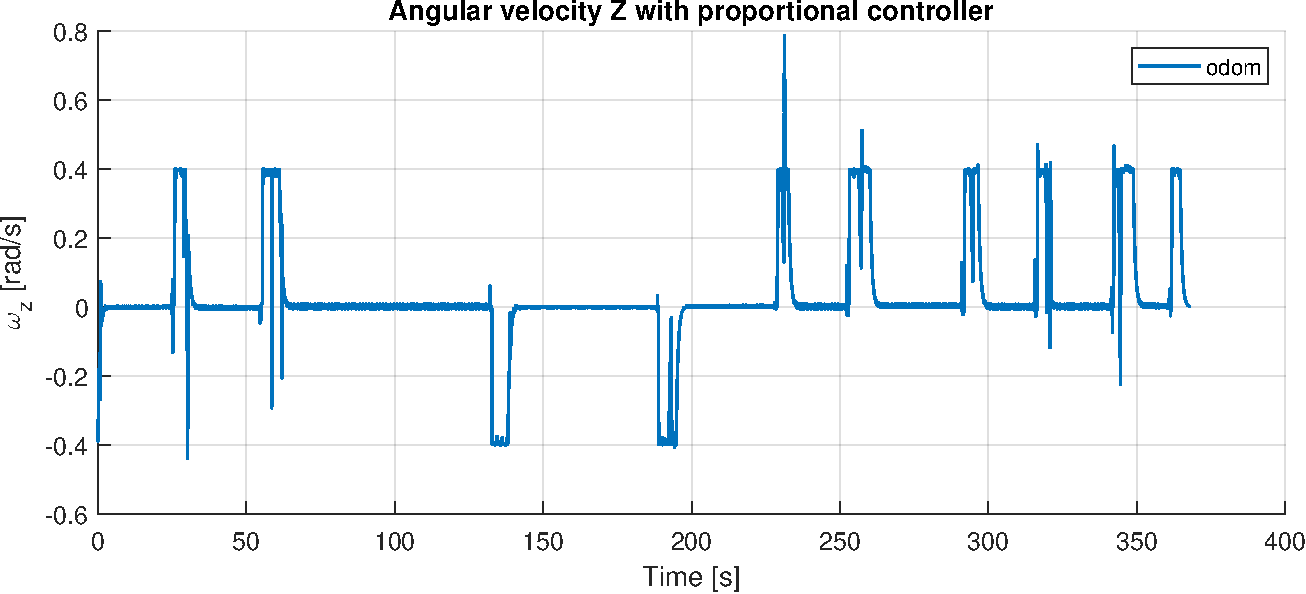
\includegraphics[width=0.7\textwidth]{./img/MATLAB/angular_velocity_proportional.pdf}
    \caption{Velocity profiles of the robot during the simulation with the proportional controller.}
    \label{fig:proportional_controller_velocity_profiles}
\end{figure}

One can also observe some severe (but luckily not too frequent) peaks in the velocities profiles that violate the constraints imposed.
Similarly to the behavior observer in previous assignment, this fact find its explanation in poor performances of the machine on which the simulation is run.
The simulation is run on a virtual machine with limited computational power, which results in some momentary oscillations in the robot's dynamics which are well captured by its telemetries.
We think that a switch to a native environment of \texttt{Ubuntu 20.04} on a \texttt{Linux} kernel machine would solve this issue.

\section{Lyapunov controller}
\label{sec:lyapunov_controller}

In this section, we proceed with the implementation of a Lyapunov-based controller for the already defined system.

Lyapunov control theory is a powerful tool for designing controllers that proofs the stability of non-linear systems.
The main idea is to find a Lyapunov function associated with the system and prove its convergence to the desired equilibrium point.
Notice that global asymptotic stability is guaranteed only if the Lyapunov function is positive definite and radially unbounded.

Once the Lyapunov function is defined and its properties are verified, we can derive a control law that ensures the system's stability.
Again, many methods from non-linear control theory exists such as the backstepping method, the feedback linearization method, or again passivation-based methods.

A final important remark here is that the control law derived from Lyapunov theory is not unique and generally speaking is also much more complex than the one derived from traditional linear control theory.
Even if stability is guaranteed, the performance of the system may not be optimal and a proper tuning of the controller is not always straightforward.


\subsection{Lyapunov control law}
\label{subsec:lyapunov_control_law}

Based on the work of \cite{lyapunov_techniques}, we can derive a Lyapunov control law for a generic unicycle-like system.
Given that the low level firmware of the \texttt{Turtlebot3} robot allows us to send control inputs in the form of linear and angular velocities, we can consider the turtlebot as a unicycle-like system and apply the Lyapunov control law to it.

\begin{figure}[H]
    \centering
    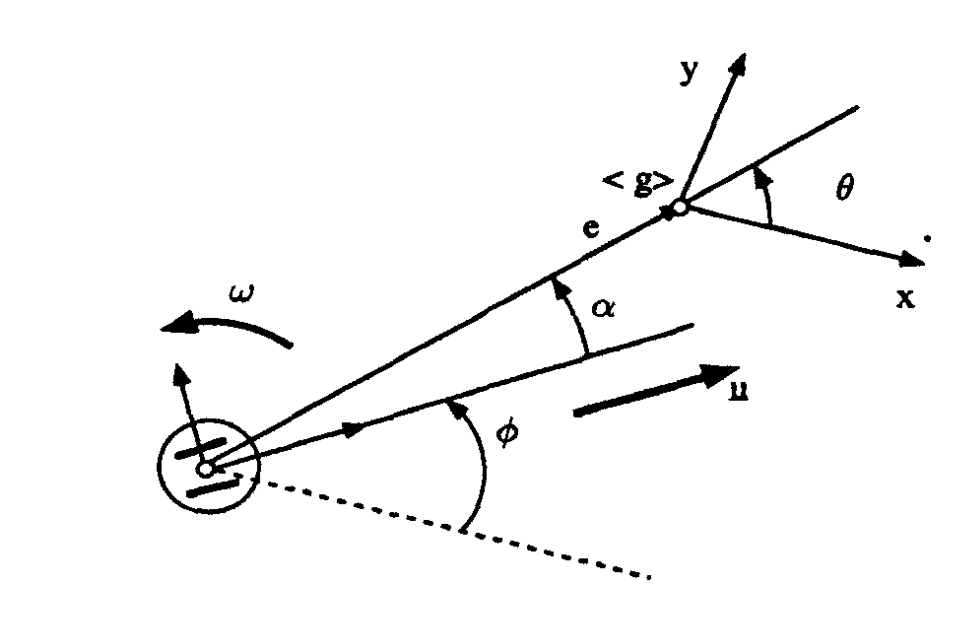
\includegraphics[width=0.7\textwidth]{./img/lyapunov_scheme.png}
    \caption{Schematic representation of the unicycle-like system and the reference frame.}
    \label{fig:lyapunov_scheme}
\end{figure}

Based on the notation used in Figure \ref{fig:lyapunov_scheme}, we can define the following Lyapunov function:

\begin{align}
    v & = k_1 \cos(\alpha) e                                                                         \\
    w & = k_2 \alpha + k_1 \frac{\sin(\alpha) \cos(\alpha)}{\alpha} \left(\alpha + k_3 \theta\right)
    \label{eq:lyapunov_control_law}
\end{align}

Where $k_1$, $k_2$, and $k_3$ are positive constants, $e$ is the Euclidean distance from the target waypoint, $\alpha$ is the angle between the robot heading and the target waypoint, and $\theta$ is the angle between the vector connecting the robot to the target waypoint and the waypoint direction (see Figure \ref{fig:lyapunov_scheme}).

It turns out that with a proper remapping of the control inputs, we can obtain a Lyapunov function that is positive definite and radially unbounded, hence ensuring the global asymptotic stability of the system.



\subsection{Implementation}
\label{subsec:lyapunov_implementation}

The code for the implementation of the Lyapunov controller is provided in the Listing \ref{lst:lyapunov_controller_code}.

\begin{lstlisting}[
    style=Matlab-editor,
    caption={Code for the implementation of the Lyapunov controller.},
    label={lst:lyapunov_controller_code}
]
function [v, w] = controlLyapunov(pos_x, pos_y, pos_yaw, target_x, target_y, target_yaw)
% This controller implements a Lyapunov-based control law for the unicycle-like
% system. It uses a Lyapunov function to derive the control inputs for the robot.
% The controller is designed to ensure global asymptotic stability of the system.
% Inspired by: Aicardi et al. (1995)

bound = @(value, limit) max(min(value, limit), -limit);

% Limits
max_linear_speed = 0.8;
max_angular_speed = 1.6;

% Gains
K_rho   = 1.0;
K_alpha = 1.5;
K_delta = 1.0;

dx = target_x - pos_x;
dy = target_y - pos_y;
rho = hypot(dx, dy);
alpha = wrapToPi(atan2(dy, dx) - pos_yaw);
theta = wrapToPi(atan2(dy, dx) - target_yaw);

% Control law (from Aicardi paper)
v = K_rho * rho * cos(alpha);
w = K_alpha * alpha + K_rho * (sin(alpha) * cos(alpha)) + K_rho * (sin(alpha) * cos(alpha)) * K_delta * theta / max(abs(alpha), 1e-3) * sign(alpha);

v = bound(v, max_linear_speed);
w = bound(w, max_angular_speed);

end
\end{lstlisting}



\subsection{Results}
\label{subsec:lyapunov_results}

The results of the obtained trajectory are shown in Figure \ref{fig:lyapunov_controller_trajectory}, where we can see the waypoints highlighted in red and the trajectory of the robot drawn in black.

\begin{figure}[H]
    \centering
    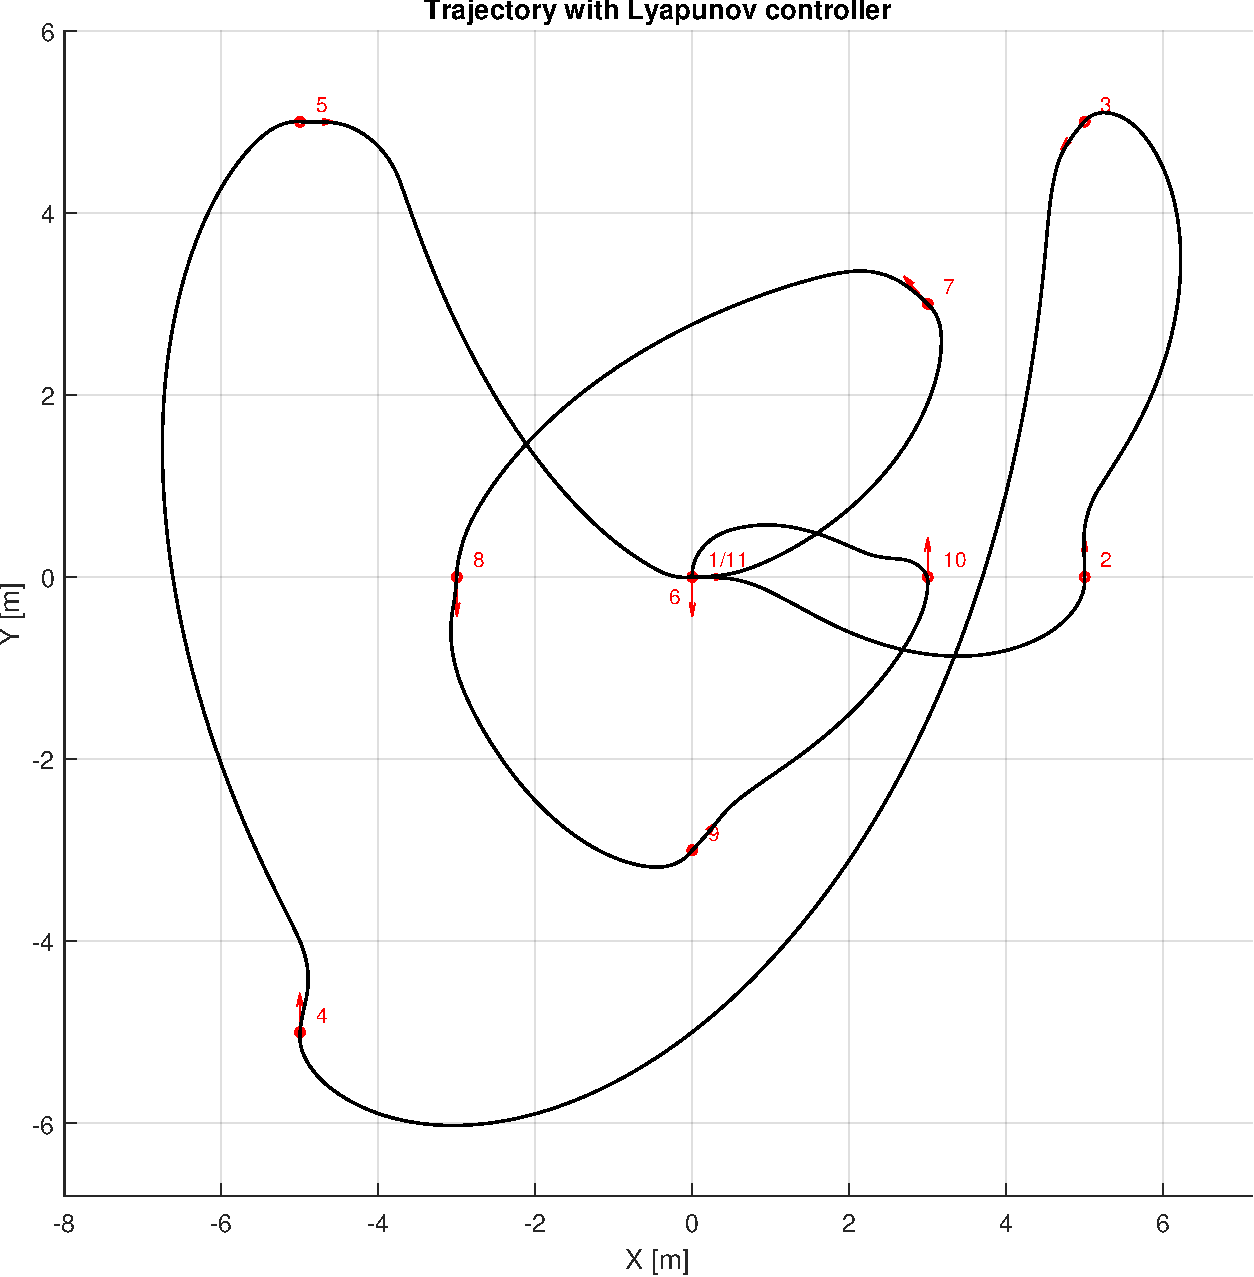
\includegraphics[width=0.6\textwidth]{./img/MATLAB/trajectory_lyapunov.pdf}
    \caption{Trajectory of the robot during the simulation with the Lyapunov controller.}
    \label{fig:lyapunov_controller_trajectory}
\end{figure}

With respect to the proportional controller, we can see that the Lyapunov controller is able to smoothly go through the waypoints and to reach them avoiding stop-and-go behavior.
The if-else logic is not needed any more given that the control law is able to smoothly connect the waypoints weighting the timing and amplitude for steering and velocity commands based on the 3 parameters $k_1$, $k_2$, and $k_3$.
One could also modify the parameters to obtain a more aggressive or conservative behavior of the robot, with consequent changes in the trajectory.

When it comes to the velocities profile, we observe that linearity is lost and non-linear behavior is present.

\begin{figure}[H]
    \centering
    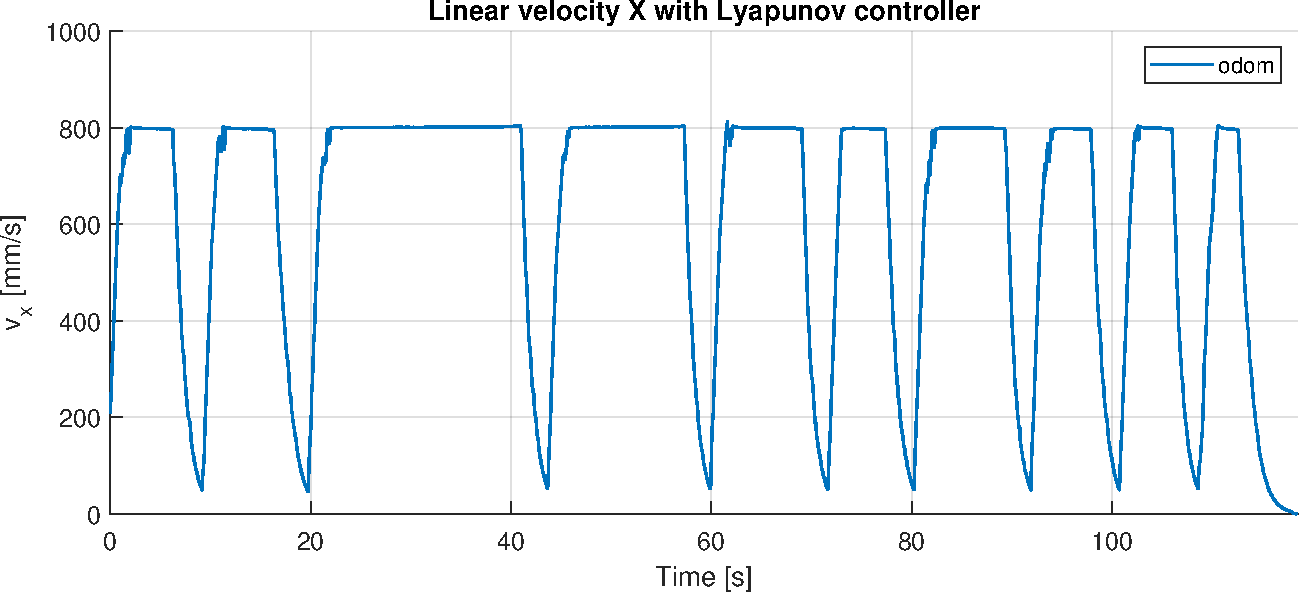
\includegraphics[width=0.7\textwidth]{./img/MATLAB/linear_velocity_lyapunov.pdf}

    \vspace{10pt}

    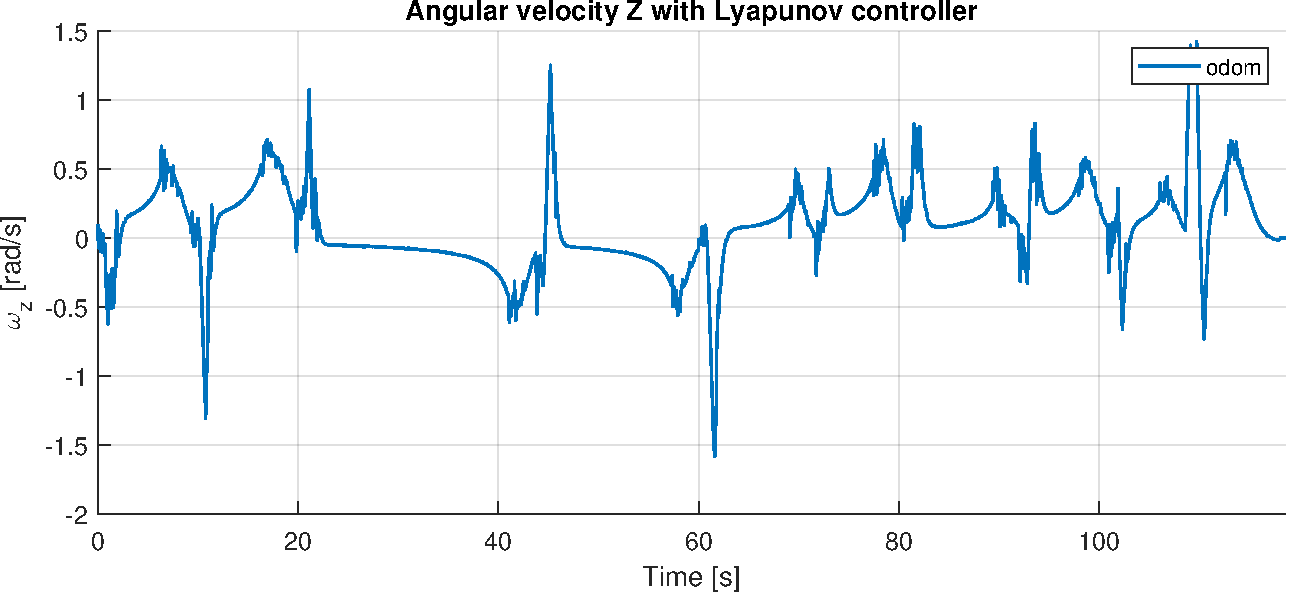
\includegraphics[width=0.7\textwidth]{./img/MATLAB/angular_velocity_lyapunov.pdf}
    \caption{Velocity profiles of the robot during the simulation with the Lyapunov controller.}
    \label{fig:lyapunov_controller_velocity_profiles}
\end{figure}

Notice that with respect to the simulation run with the proportional controller, the linear velocity is now not limited to $0.2 \text{[ m/s]}$, but it can reach up to $0.8 \text{[ m/s]}$, and similarly the angular velocity can reach up to $1.6 \text{[ rad/s]}$.
The author has decided to increase the limits of the velocities in order to allow the robot to reach the waypoints in a shorter time.
Nevertheless, the no-slip condition generally required for the unicycle-like system has been checked and verified even with the presence of stronger inertial forces due to the higher velocities.

\section{Conclusions}
\label{sec:conclusions}

In this short report, we have presented the results of the second assignment of the course on Autonomous Vehicles.
We have shown how to implement a feedback control strategy for a mobile robot, specifically the \texttt{Turtlebot3} robot, in a simulated environment using \texttt{ROS1} and \texttt{Gazebo}.

Even if not extensively discussed in this report, the \texttt{Simulink} system has allowed to easily load waypoints from different sources (i.e. workspace or ROS topic) and no differences in the results have been observed.

Most importantly, we have shown how to implement a simple proportional controller and a Lyapunov-based controller for the robot.
While both have shown to be effective in guiding the robot to the target waypoints, the Lyapunov controller has demonstrated a native smoothness in the trajectory, avoiding stop-and-go behavior.

Some unwanted spikes in the telemetry of the robot have been observed during the simulation, which could be due to the fact that the simulation was run on a \texttt{Windows} environment.
Further investigations and testing could be done by switching to a native \texttt{Linux} environment, which could provide better performance and more accurate results.

\vspace*{\fill}
\nocite{*}
\bibliographystyle{plain}
\bibliography{references.bib}

\end{document}
